\documentclass[a4paper]{article}

\usepackage[T1]{fontenc}

\usepackage[spanish, es-nodecimaldot, es-noquoting]{babel}
%\usepackage{icomma} % Use dot as decimal separator
\usepackage{booktabs} % For better-looking tables
\usepackage{wrapfig}
\usepackage{caption}
%\usepackage{siunitx}


\usepackage{refcount}

\usepackage{multicol}
\usepackage{mathtools}

\usepackage[normalem]{ulem}

\pagestyle{empty}

\usepackage{pgf,tikz}
\usepackage{pgfplots}
\usetikzlibrary{matrix}
\usetikzlibrary{arrows}
\usetikzlibrary{babel}


\parindent 0pt
\setlength{\parskip} {1ex plus 0.5ex minus 0.2ex}

\usepackage{amsfonts}

%\DeclareSymbolFontAlphabet{\mathbb}{AMSb}
%\DeclareSymbolFontAlphabet{\mathbbl}{bbold}

\newcommand{\Sym}{{\mathcal S}}
\DeclareMathOperator{\Aut}{Aut}
\DeclareMathOperator{\Tr}{Tr}
\DeclareMathOperator{\trace}{Trace}
\DeclareMathOperator{\range}{range}
\DeclareMathOperator{\rank}{rank}

\usepackage{breqn}
\usepackage{multicol}
\usepackage{colortbl}
\usepackage{lmodern}
\usepackage{tabularx}
\usepackage{multirow}
\usepackage{amssymb}
\usepackage{amsmath}
\usepackage{stmaryrd}
\usepackage{color}
\usepackage{graphicx}
\graphicspath{ {img/} }
\usepackage{hyperref}

\input{epsf}

\DeclareMathOperator{\Hom}{Hom}
\DeclareMathOperator{\sing}{sing}

\DeclareMathOperator{\var}{var}
\DeclareMathOperator{\cov}{cov}
\DeclareMathOperator{\corr}{corr}

\DeclareMathOperator{\chara}{char}
\DeclareMathOperator{\Jacob}{Jacob}
\DeclareMathOperator{\Sing}{Sing}
\newcommand{\fracNoLine}[2]{\genfrac{}{}{}{0pt}{#1}{#2}}

%\beamerdefaultoverlayspecification{<+->}

\usepackage{listings,xcolor,bm}


\definecolor{mygreen}{rgb}{0,0.6,0}
\definecolor{mygray}{rgb}{0.5,0.5,0.5}
\definecolor{mymauve}{rgb}{0.58,0,0.82}
\lstset{
  backgroundcolor=\color{white},   % choose the background color; you must add
  basicstyle=\small\ttfamily,      % the size of the fonts that are used for the code
  breakatwhitespace=false,         % sets if automatic breaks should only happen at whitespace
  breaklines=true,                 % sets automatic line breaking
  captionpos=b,                    % sets the caption-position to bottom
  commentstyle=\color{mygreen},    % comment style
  deletekeywords={...},            % if you want to delete keywords from the given language
  escapeinside={\%*}{*)},          % if you want to add LaTeX within your code
  extendedchars=true,              % lets you use non-ASCII characters; for 8-bits encodings only, does not work with UTF-8
  firstnumber=1,                % start line enumeration with line 1000
  frame=single,	                   % adds a frame around the code
  keepspaces=true,                 % keeps spaces in text, useful for keeping indentation of code (possibly needs columns=flexible)
  keywordstyle=\color{blue},       % keyword style
  language=Python,                 % the language of the code
  morekeywords={*,...},            % if you want to add more keywords to the set
  numbers=left,                    % where to put the line-numbers; possible values are (none, left, right)
  numbersep=5pt,                   % how far the line-numbers are from the code
  numberstyle=\tiny\color{mygray}, % the style that is used for the line-numbers
  rulecolor=\color{black},         % if not set, the frame-color may be changed on line-breaks within not-black text (e.g. comments (green here))
  showspaces=false,                % show spaces everywhere adding particular underscores; it overrides 'showstringspaces'
  showstringspaces=false,          % underline spaces within strings only
  showtabs=false,                  % show tabs within strings adding particular underscores
  stepnumber=5,                    % the step between two line-numbers. If it's 1, each line will be numbered
  stringstyle=\color{mymauve},     % string literal style
  tabsize=4,	                   % sets default tabsize to 2 spaces
  title=\lstname                   % show the filename of files included with \lstinputlisting; also try caption instead of title
}


\newtheorem{prop}{Proposici\'on}
\newtheorem{algo}[prop]{Algoritmo}
\newtheorem{teor}[prop]{Teorema}
\newtheorem{lema}[prop]{Lema}
\newtheorem{coro}[prop]{Corolario}
\newtheorem{defi}[prop]{Definici\'on}

\newcommand{\ideal}[1]{{\left\langle{#1}\right\rangle}}
\newcommand{\demo}{\textbf {Demostraci\'on. }}
\newcommand{\obse}{\textbf {Observaci\'on. }}
\newcommand{\Input}{\textbf {Input: }}
\newcommand{\Output}{\textbf {Output: }}
\newcommand{\Examp}{\textbf {Ejemplo }}
\newcommand{\Examps}{\textbf {Ejemplos }}

\newcommand{\kk}{{\mathbbl k}}
\newcommand{\V}{{\mathbf V}}
\newcommand{\I}{{\mathbf I}}
\newcommand{\PP}{{\tilde P}}
\newcommand{\QQ}{{\tilde Q}}

\newcommand{\F}{{\mathbb F}}
\newcommand{\Q}{{\mathbb Q}}
\newcommand{\N}{{\mathbb N}}
\newcommand{\R}{{\mathbb R}}
\newcommand{\Z}{{\mathbb Z}}
\newcommand{\CC}{{\mathbb C}}
\newcommand{\eLL}{{\mathcal L}}


\newcommand{\Id}{\textrm {Id}}


\newcommand{\MinAss}{\textrm {MinAss}}
\newcommand{\Ass}{\textrm {Ass}}
\newcommand{\mcm}{\textrm {mcm}}
\newcommand{\mcd}{\textrm {mcd}}
%\newcommand{\mod}{\textrm { mod }}
\newcommand{\lt}{\textrm {lt}}
\newcommand{\Lt}{\textrm {Lt}}
\newcommand{\lp}{\textrm {lp}}
\newcommand{\lc}{\textrm {lc}}
\newcommand{\lm}{\textrm {lm}}
\newcommand{\barra}{\ /\ }
\newcommand{\multideg}{\textrm {multideg}}

\newcommand{\sep}{\textrm {sep}}
\newcommand{\Syz}{\textrm {Syz}}
\newcommand{\n}{\~n}
\newcommand{\cG}{\textrm {cG}}
\newcommand{\dG}{\textrm {dG}}
\newcommand{\nG}{\textrm {nG}}
\newcommand{\CE}{\textrm {CE}}
\newcommand{\CG}{\textrm {CG}}
\newcommand{\CF}{\textrm {CF}}
\newcommand{\DG}{\textrm {DG}}
\renewcommand{\NG}{\textrm {NG}}

\newcommand{\p}{{\boldsymbol{p}}}
\newcommand{\q}{{\boldsymbol{q}}}

\newcommand{\X}{{\boldsymbol{X}}}
\newcommand{\x}{{\boldsymbol{x}}}
\renewcommand{\u}{{\boldsymbol{u}}}
\renewcommand{\t}{{\boldsymbol{t}}}
\renewcommand{\a}{{\boldsymbol{a}}}
\renewcommand{\b}{{\boldsymbol{b}}}
\renewcommand{\c}{{\boldsymbol{c}}}

%Titulos en espa�ol
%\renewcommand{\chaptername}{Cap\'{\i}tulo}
%\renewcommand{\bibname}{Bibliograf\'{\i}a}

\newcommand{\kring}{\kk[\x]}
\newcommand{\kRing}{\kk[X]}
\newcommand{\qring}{\Q[\x]}

%\renewcommand\itemindent{-10pt}
%\renewcommand{\theenumi}{\arabic{enumi}}
%\renewcommand{\labelenumi}{\Alph{enumi}}

\definecolor{issac}{rgb}{1.00,0.00,0.00}
%------------------------------------------------------------------

\title{Componentes principales}


\author{Santiago Laplagne}

\begin{document}

\maketitle

\section{Introducci\'on}

En estas notas desarrollamos los conceptos teóricos de álgebra lineal detrás del análisis de componentes principales.

\subsection{Qué es el análisis de comonentes principales (PCA)}

\begin{itemize}
    \item PCA es un método de \emph{aprendizaje no supervisado} para reducir la dimensionalidad de un conjunto de datos.
    \item Identifica las direcciones (componentes principales) que explican la mayor parte de la variabilidad en los datos.
    \item Las componentes principales son combinaciones lineales de las variables originales.
\end{itemize}

\begin{center}
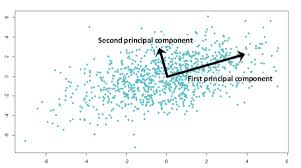
\includegraphics[scale=0.5]{dosComponentes.jpg}
\end{center}

\subsection{Ejemplo}

\begin{itemize}
\item Si tenemos un conjunto de datos con 3 variables pero hay dependencia lineal entre las variables (es decir, $a x_1 + b x_2 + c x_3 \approx 0$), al representar a los puntos en el espacio, todos los puntos quedaran ubicados cerca de un plano (el plano $a x_1 + b x_2 + c x_3 = 0$).
\item Si proyectamos los puntos sobre ese plano, y consideramos nuevas variables definidas por las coordenadas de las proyecciones en ese plano, estaremos representando las 3 variables originales utilizando solo 2 variables, sin perder mucha información.
\end{itemize}

\section{Varianza, covarianza y correlación}

\subsection{Varianza.}
Ya vimos la f\'ormula de varianza para una variable $x = (x_1, x_2, \dots, x_n)$:
$$
\var(x) = \frac{\sum_{i=1}^n(x_i - \bar x)^2}{n},
$$
donde $\bar x = \frac{\sum_{i = 1}^n x_i}{n}$ es el promedio o la media de los valores de $x$.

Recordemos la definición de producto interno entre vectores:
$$\langle x, y\rangle = x_1 y_1 + x_2 y_2 + \dots + x_n y_n = \begin{pmatrix} x_1 & x_2 & \cdots & x_n \end{pmatrix} \begin{pmatrix} y_1 \\ y_2 \\ \vdots \\ y_n \end{pmatrix} = x^T y,$$
donde usamos la convención de representar a los vectores como matrices columna.

Usando productos internos podemos escribir
$$
\var(x) = \frac{\langle x - \bar x,  x - \bar x \rangle}{n} = \frac{\| x - \bar x\|^2}{n}.
$$


\subsection{Covarianza.} Definimos ahora la covarianza entre dos variables $x = (x_1, x_2, \dots, x_n)$ e $y = (y_1, y_2, \dots, y_n)$ que mide la relaci\'on entre ellas:
$$
\cov(x,y) = \frac{\sum_{i = 1}^n (x_i - \bar x)(y_i - \bar y)}{n}= \frac{\langle x - \bar x , y - \bar y \rangle}{n}
$$

\textbf{Interpretaci\'on:}
\begin{itemize}
\item Si $(y_i - \bar y)$ es siempre positivo cuando $(x_i - \bar x)$ es positivo, la covarianza será grande positiva.
\item Si uno es siempre positivo cuando el otro es negativo, la covarianza será grande negativa.
\end{itemize}

\subsection{Correlaci\'on.} Dividiendo la fórmula de covarianza por los desvíos de cada variable obtenemos la fórmula de correlación:
$$
\corr(x,y) = \frac{\cov(x, y)}{\sqrt{\var(x)}\sqrt{\var(y)}} = \frac{\cov(x, y)}{\sigma(x)\sigma(y)}
$$

Podemos reescribir esta fórmula:
$$
\corr(x,y) = \frac{\frac{\sum_{i = 1}^n (x_i - \bar x)(y_i - \bar y)}{n}}{\frac{\|x  - \bar x\|}{\sqrt{n}}\frac{\|y - \bar y\|}{\sqrt{n}}} = \frac{\langle x - \bar x, y - \bar y\rangle}{\|x - \bar x\|\|y  - \bar y\|},
$$

\subsection{\'Angulos y correlaci\'on}

\begin{minipage}{.45\textwidth}
Recordemos la fórmula para el ángulo entre dos vectores:
$$
\cos(\theta) = \frac{\langle x, y \rangle}{\|x\|\|y\|}
$$
\end{minipage} \hspace{.4cm} %
\begin{minipage}{.45\textwidth}
\begin{tikzpicture}[scale = 0.7]
% Draw the origin
\coordinate (O) at (0,0);

% Define the vectors x and y
\coordinate (X) at (4,0);
\coordinate (Y) at (3,3);

% Draw the vectors
\draw[->, thick] (O) -- (X) node[anchor=north east] {$x$};
\draw[->, thick] (O) -- (Y) node[anchor=south west] {$y$};

% Draw the angle theta
\draw (1,0) arc (0:45:1) node[midway, anchor = west] {$\theta$};

% Optional: Draw the axes
\draw[->] (-1,0) -- (5,0) node[anchor=north west] {};
\draw[->] (0,-1) -- (0,4) node[anchor=south east] {};

\end{tikzpicture}
\end{minipage}

La correlación
$$\corr(x, y) = \frac{\langle x - \bar x, y - \bar y \rangle}{\|x - \bar x\|\|y - \bar y\|}$$
 es el coseno del ángulo entre $x - \bar x$ e $y - \bar y$.

\begin{itemize}
\item Si el ángulo es $0^\circ$, la correlación es 1.
\item Si el ángulo es $180^\circ$, la correlación es -1.
\item Si el ángulo es $90^\circ$, la correlación es 0.
\end{itemize}

\subsection{Matriz de Covarianza}

Consideramos ahora una matriz de datos $X \in \R^{N \times p}$, donde las $p$ columnas representan distintas variables y las $N$ filas, observaciones.
\begin{itemize}
    \item La matriz de covarianza mide la relación lineal entre dos o más variables.
    \item Dada una matriz de datos \( X \) de \( N \) observaciones y \( p \) variables, la matriz de covarianza \( \Sigma \) se define como:
    \[
    \Sigma = \frac{(X - \bar X)^T (X - \bar X)}{N} \in \R^{p \times p},
    \]
    donde la matriz $\bar X$ tiene en cada columna el valor medio de la columna correspondiente de $X$.
    \item Si llamamos $X^\star$ a la matriz con datos normalizados $X^\star = X - \bar X$,
    $$\boxed{\Sigma = \frac{(X^\star)^T X^\star}{N}}$$

    \item Las columnas de $X^\star$ son las columnas originales de $X$ normalizadas a media $0$.
    \item Cada elemento $\Sigma_{ij}$ en la matriz de covarianza representa la covarianza entre las variables $x^i$ y $x^j$,
    $$\cov(x^i, x^j) = \frac{\sum_{k = 1}^N (x_k^i - \overline{x^i})(x_k^j - \overline{x^j})}{N}  = \frac{\langle x^i - \overline{x^i}, x^j - \overline{x^j} \rangle}{N} = {\Sigma}_{ij}.$$
\end{itemize}

\section{Aspectos geométricos}

\subsection{Proyección de un punto sobre una recta}

Para construir las componentes principales, proyectamos los datos sobre rectas y buscamos la recta para la cual se maximiza la varianza.

\begin{center}
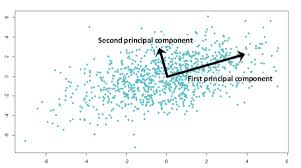
\includegraphics[scale=0.5]{dosComponentes.jpg}
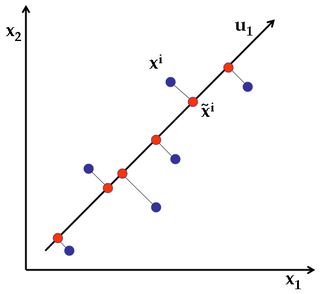
\includegraphics[scale=0.3]{projection.png}
\end{center}

\subsection{Longitud de la proyección }

\begin{minipage}{.6\textwidth}
La longitud de la proyecci\'on de un vector $u$ sobre la recta generada por un vector $v$ es
$$longitud = \|u\| \cos(\theta) = \frac{\langle u, v \rangle}{\|v\|}.$$

Si $\|v\| = 1$ (vector unitario), obtenemos $$longitud = \langle u, v \rangle.$$

\end{minipage} \hspace{.2cm} %
\begin{minipage}{.35\textwidth}
\begin{center}
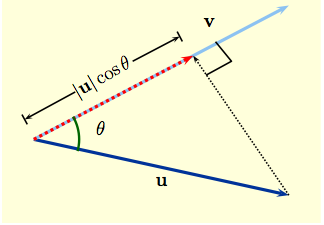
\includegraphics[scale=0.25]{vectors08.png}
\end{center}

\end{minipage} \hspace{.4cm} %

\subsection{Proyección de un conjunto de datos}

Si tenemos una matriz de datos $X \in \R^{N \times p}$, el vector de proyecciones sobre $v = (v_1, v_2)$ (unitario) ser\'a simplemente $Xv$.

Si $X$ tiene dos columnas,
$$
Xv =
\begin{pmatrix} x^1_1 & x^2_1 \\ x^1_2 & x^2_2 \\ \vdots & \vdots \\ x^1_n & x^2_n \end{pmatrix}
\begin{pmatrix} v_1 \\ v_2 \end{pmatrix} =
\begin{pmatrix} x^1_1 \cdot v_1 + x^2_1 \cdot v_2 \\ x^1_2 \cdot v_1 + x^2_2 \cdot v_2 \\ \vdots \\ x^1_n \cdot v_1 + x^2_n \cdot v_2 \end{pmatrix} =
\begin{pmatrix} \langle (x^1_1, x^2_1), (v_1, v_2) \rangle \\ \langle (x^1_2, x^2_2), (v_1, v_2) \rangle  \\ \vdots \\ \langle (x^1_n, x^2_n), (v_1, v_2) \rangle \end{pmatrix}.
$$

\textbf{Ejemplo.} Para proyectar los datos sobre el eje $x_1$, multiplicamos la matrix $X$ por el vector canónico $(1,0)$ y obtenemos la primera columna de la matriz $X$.

\subsection{Varianza de las proyecciones}

Si trabajamos con $X^\star$ (datos normalizados), las variables tienen media 0, y las proyecciones sobre una recta también tendrán media 0 (ejercicio).

Por lo tanto, podemos calcular la varianza de la proyección sobre la recta generada por $v$ por la fórmula:
$$
\var(X^\star v) = \frac{\langle X^\star v, X^\star v \rangle}{n} = \frac{(X^\star v)^T (X^\star v)}{n} = \frac{v^T (X^\star)^T X^\star v}{n} = v^T \left(\frac{(X^\star)^T X^\star}{n}\right) v.
$$

¡Apareció la matriz de covarianza!

$$
\var(X^\star v) = v^T \Sigma v
$$


\section{Componentes principales}

\subsection{Primera componente}
Para encontrar la dirección en la que las proyecciones tienen mayor varianza, debemos encontrar el vector $v$ que maximiza
$$v^T \Sigma v.$$

Repasamos algunas definiciones y teoremas de álgebra lineal. Para un desarrollo más completo, ver Sección 5.5 del Apunte de \'Algebra Lineal Computacional (\url{https://github.com/slap/ALC-apunte}).


\begin{defi}\hfill
\begin{enumerate}
\item Decimos que una matriz $A \in \R^{n \times n}$ es \emph{simétrica} si $A = A^T$ (equivalentemente, $a_{ij} = a_{ji}$ para todo $1 \le i, j \le n$).
\item Si una matriz $A \in \R^{n \times n}$ es simétrica y $v^T A v \ge 0$ para todo $v \in \R^n$, decimos que $A$ es \emph{semidefinida positiva}. Si $v^T A v > 0$ para todo $v \in \R^n$ decimos que $A$ es \emph{definida positiva}.
\end{enumerate}
\end{defi}

\begin{prop}\hfill
\begin{enumerate}
\item Si $A \in \R^{n \times n}$ es simétrica, entonces $A$ es diagonalizable, admite una base ortonormal de autovectores y todos los autovalores de $A$ son reales. Es decir, existe una matriz $U \in \R^{n \times n}$ unitaria ($U^T U = \Id$) tal que
    $$
    A = U D U^T,
    $$
donde $D$ es una matriz diagonal con los autovalores de $A$ en la diagonal. Las columnas de $U$ son los autovectores de $A$.
\item Adicionalmente, si $A \in \R^{n \times n}$ es semidefinida positiva, todos los autovalores de $A$ son no-negativos.
\item Si $A \in \R^{n \times n}$ es definida positiva, todos los autovalores de $A$ son no-negativos.
\end{enumerate}
\end{prop}

\textbf{Observación.} Si $A$ es definida positiva, todos sus autovalores son positivos y por lo tanto $A$ es inversible.

\begin{prop}
Si $A \in \R^{n \times p}$ ($n > p$) y definimos $X = A^T A \in \R^{p \times p}$, entonces $X$ es semidefinida positiva.

Si las columnas de $A$ son linealmente independientes (es decir $A$ tiene rango $p$), entonces $X$ es definida positiva.
\end{prop}


Utilizando estos resultados, se puede probar que el vector $v$ que maximiza $v^T \Sigma v$ es el autovector de $\Sigma$ correspondiente al mayor autovalor.

Este vector $v$ es la dirección de la primera componente principal.

\subsection{¿Cómo calculamos las demás componentes?}

Elegimos las direcciones de forma tal que
\begin{itemize}
\item la proyección en la primer dirección tenga la mayor varianza,
\item la proyección en la segunda dirección tenga la segunda mayor varianza,
\item y así siguiendo,
\end{itemize}
con la condición adicional de que las direcciones sean perpendiculares. Esto implica que la información contenida en cada proyección sea independiente de las demás proyecciones.

\textbf{Obtenemos:} Las siguientes direcciones corresponden a los autovectores de la matriz de covarianza correspondientes a los demás autovalores ordenados de mayor a menor.

\subsection{Cálculo de PCA paso a paso}

A partir de la matriz de covarianza, podemos calcular las componentes principales de la siguiente forma.

    \begin{enumerate}
        \item Calculamos la matriz $X^\star = X - \bar X$ de datos normalizados.
        \item Calculamos la matriz de covarianza $\Sigma = \frac{(X^\star)^T X^\star}{n} \in \R^{p \times p}$.
        \item Calculamos los autovalores de $\Sigma$: $\lambda_1 \ge \lambda_2 \ge  \dots \ge \lambda_p \ge 0$ y los correspondientes autovectores $u_1, \dots, u_p$ (de norma 1).

        \item Definimos las nuevas variables $z_i = X^\star u_i$ (las proyecciones de los datos sobre las direcciones principales).
        \item Si $U$ es la matriz de autovectores, el nuevo conjunto de datos es $Z = X^\star U$ (las nuevas variables son las columnas de $Z$).
    \end{enumerate}

\subsection{Relación entre autovectores y componentes principales}
\begin{itemize}
    \item Los autovectores de la matriz de covarianza definen las direcciones de las componentes principales.
    \item Los autovalores indican la cantidad de varianza explicada por cada componente principal.
    \item Las componentes principales se obtienen proyectando los datos sobre estos autovectores:
\[
Z = X^\star U
\]
donde $Z$ son las componentes principales, \( {X} \) es la matriz de datos y \( {U} \) es la matriz de autovectores.
\end{itemize}

\subsection{Varianza explicada}
\begin{itemize}
    \item Los autovalores indican la cantidad de varianza explicada por cada componente principal.
\end{itemize}

\textbf{Ejemplo:} Si los autovalores de la matriz de covarianza son
$$
\lambda_1 = 30, \lambda_2 = 8, \lambda_3 = 2,
$$
definimos la varianza total como la suma $\lambda_1 + \lambda_2 + \lambda_3 = 30 + 8 + 2 = 40$.

El porcentaje explicado por cada componente sera el valor de cada autovalor dividido por la varianza total.

Los porcentajes de varianza explicada son
$$\frac{30}{40} = 0.75, \frac{8}{40} = 0.2 \text{ y } \frac{2}{40} = 0.05.$$

\subsection{Varianza explicada acumulada}

Los porcentajes de varianza explicada son
$$\frac{30}{40} = 0.75, \frac{8}{40} = 0.2 \text{ y } \frac{2}{40} = 0.05.$$

Si consideramos las dos primeras componentes, tendremos un total de varianza explicada
$$0.75 + 0.2 = 0.95.$$

Es decir, que si utilizamos las dos primeras componentes, perdemos solo un $5\%$ de información.

De esta forma podemos reducir la dimensión de los datos, podemos quedarnos con solo estas dos componentes sin perder mucha información.

\subsection{Ventajas de PCA}
\begin{itemize}
    \item Reducción de dimensionalidad: Permite trabajar con menos variables sin perder mucha información.
    \item Eliminación de redundancia: Los componentes principales son ortogonales entre sí, eliminando la multicolinealidad.
    \item Mejora del rendimiento de los algoritmos: Menos variables pueden resultar en tiempos de computación más rápidos.
\end{itemize}

\end{document}

%------------------------------------------------------------------

